\documentclass{article}
\usepackage[utf8]{inputenc}
\usepackage{tikz}
\usepackage{verbatim}

\usepackage[utf8]{inputenc}
\renewcommand{\arraystretch}{1.5}
 

\setlength{\parindent}{0em}
\setlength{\parskip}{1em}

\title{Flow Synthetic Assets Working Paper}
\author{Antonia Chen}
\date{September 2019}

\usepackage{natbib}
\usepackage{graphicx}

\usetikzlibrary{arrows,calc}
\usepackage{relsize}

\begin{document}

\maketitle

\section{Introduction}
A new type of fungible Cryptocurrency - stablecoin of Euro  (\textbf{\textit{fEUR}}) is created by our \textbf{\textit{Flow}} protocol, to meet the DeFi market demand of stablecoins for non-USD currencies. Stablecoins of other currencies such as JPY will be created in the future.  

\section{Liquidity Pool}
A liquidity provider can run his/her own liquidity pool after depositing USD stablecoins to be used as collateral to open positions when new fEUR tokens are minted. Flow protocol support co-existence of multiple liquidity pools. 

\section{Model Setup}
The following model allows any trader to purchase  (\textbf{\textit{fEUR}}) with USD stablecoins through the protocol. 

\begin{itemize}

  \item $t$ - Time
  
  \item $m$ - Midpoint of Market Exchange Rate\\
  $m_0$ - Midpoint of Market Exchange Rate at opening of a position\\
  $m_t$ - Midpoint of Market Exchange Rate at time $t$
  
  \item $\theta$ - Market Fluctuation\\
  $m_t=m_0(1+\theta_t)$ for any particular open position

  \item $b$ and $a$ -  Bid or Ask spread between the Flow bid price $m_t(1-b)$ or ask price $m_t(1+a)$ to the market midpoint $m_t$ set by the liquidity provider of a pool that
  
  $$b_t=\frac{m_t-m_t(1-b)}{m_t}$$

  $$a_t=\frac{m_t(1+a)-m_t}{m_t}$$
  
  Bid and ask spread $b_t$ and $a_t$ are chosen by the liquidity provider that can be changed anytime. 

  \item $v$ -  Number of fEUR token issued at opening of a position
  
  \item $\alpha$ - Ratio of extra collateral required to open an position for minting any fEUR token, e.g. 10\%. To mint $v$ fEUR tokens when market exchange rate is $m_0$, $\alpha m_0v$ unit of USD stablecoins are required to be locked on top of $m_0 v$ in a liquidity pool as collateral against market fluctuations. 

  \item $c$ - Collateral of an open position that belong to the liquidity provider\\
  For $v$ fEUR tokens issued, $c_0=\alpha m_0v$, $c_t=(1+\alpha)m_0v - m_tv$. 

  \item $\beta$ - Liquidation Threshold, e.g. 5\%

  \item $\gamma$ - Extreme threshold, e.g. 1\%

  \item $\mu$ - Ratio of Liquidity Provider's collateral to the current value of fEUR at an open position, $\mu_0=\alpha$ and
  $$ \mu_t=\frac{\alpha - \theta_t}{1+\theta_t}$$

  \item $\lambda$ - Represent how far away the current Liquidity Provider's collateral ratio is from the Liquidation Threshold, $$\lambda_t=\beta-\mu_t$$
  
  \item $\delta$ - Proportion of Liquidity Provider's collateral to be given to the liquidator if a position is liquidated, 
  $$ \delta_t=\frac{\lambda_t}{\beta-\gamma}=\frac{\beta-\mu_t}{\beta-\gamma}$$
  
 \end{itemize}

\section{Mint Token \& Open Position}
Suppose a trader is interested in purchasing $v$ unit of fEUR tokens when market exchange rate midpoint is $m_0$, he/she deposits unit of $m_0(1+a_0)v$ USD stablecoins into a liquidity pool, $v$ unit of fEUR tokens are minted by Flow protocol after the liquidity provider of the pool opens a position by locking the fund as collateral
$$\{ m_0v  \quad +  \quad \alpha*m_0v \}$$

\begin{itemize}
    
    \item $m_0v$ represents the current value of $v$ unit of fEUR tokens in USD
    
    \item $\alpha*m_0 v$ is the collateral against market fluctuation that belong to the liquidity provider, made of the spread part deposited by the trader $ a_0 m_0 v$, and the rest deposited by the liquidity provider $(\alpha-a_0)m_0v$
   
    \item total value of the position equals to  $m_0v + \alpha*m_0v = (1+\alpha)m_0 v$

\end{itemize}

\section{Burn Token \& Close Position}
Suppose a trader is interested in selling $v$ unit of fEUR tokens back to the liquidity pool when market exchange rate midpoint is $m_t$, he/she deposits the fEUR tokens into a liquidity pool, $v$ unit of fEUR tokens are burnt by Flow protocol after the liquidity provider of the pool closes the open position for the $v$ unit of fEUR tokens and transfers $m_t(1-b_t)v$ unit of USD stablecoins to the trader, and all remaining collateral of the position now belong to the liquidity provider and are returned into the pool. 

\subsection{Trader sells immediately after opening position}
Suppose trader wants to sell the token back to the liquidity pool immediately after buying $v$ unit of fEUR tokens when market exchange rate midpoint is $m_0$, he receives $(1-b_0)m_0 v$ USD stablecoins back and makes loss of $-(a_0+b_0) m_0 v$ USD stablecoins. \par

Liquidity provider closes the open position $\{ m_0v \quad  +  \quad \alpha*m_0v \}$,  $\alpha m_0 v$ collateral is released and returned to the pool, together with profit made from bid spread, he makes profit of $(a_0+b_0) m_0 v$ USD stablecoins. \par

And $v$ unit of fEUR tokens are then burnt by Flow protocol.

\subsection{Trader sells fEUR when EUR/USD $\downarrow$}
Suppose EUR/USD goes down after opening of a position for $v$ fEUR tokens minted, i.e. $\theta_t<0$ and $m_t<m_0$, the position is now
$$\{ m_t v   \quad +  \quad  [(1+\alpha)m_0-m_t]v \}$$
$$\{ (1+\theta_t)m_0 v   \quad +  \quad  (\alpha-\theta_t)m_0 v \}$$
where $(\alpha-\theta_t)m_0 v$ belong to the liquidity provider. \par

If trader chooses to sell $v$ fEUR tokens back to the Liquidity pool, he receives $(1+\theta_t -b_t)m_0 v$ USD stablecoins back and makes loss of  $(\theta_t -(a_0+b_t))m_0 v$ USD stablecoins.\par

Liquidity provider closes the open position $\{ (1+\theta_t)m_0 v   \quad +  \quad  (\alpha-\theta_t)m_0 v \}$, \\ $(\alpha-\theta_t)m_0 v$ collateral is released and returned to the pool, together with profit made from bid spread, he makes profit of $((a_0+b_t) - \theta_t)m_0 v$ USD stablecoins. \par

And $v$ unit of fEUR tokens are then burnt by Flow protocol.

\subsection{Trader sells fEUR when EUR/USD $\uparrow$}
Suppose EUR/USD goes up after opening of a position for $v$ fEUR tokens minted, i.e. $\theta_t>0$ and $m_t>m_0$, the position is now
$$\{ m_t v   \quad +  \quad  [(1+\alpha)m_0-m_t]v \}$$
$$\{ (1+\theta_t)m_0 v   \quad +  \quad  (\alpha-\theta_t)m_0 v \}$$
where $(\alpha-\theta_t)m_0 v$ belong to the liquidity provider. \par

The ratio of collateral that belongs to the liquidity provider to the current value of $v$ fEUR tokens
$$ \mu_t=\frac{(\alpha-\theta_t)m_0 v}{(1+\theta_t)m_0 v}=\frac{\alpha - \theta_t}{1+\theta_t}$$\par

When EUR/USD goes high enough ($\theta_t$ large enough), there is a risk that the current value of the fEUR tokens in USD stablecoins may exceed total collateral locked in the position, i.e. $(1+\theta_t)m_0 v> (1+\alpha)m_0 v$,  in which case the liquidity provider will not be able to provide enough USD stablecoins if a trader tries to sell fEUR tokens back. A liquidity provider may choose to add more USD stablecoins into the open position to top up his collateral to increase $\mu$. While if he fails to top up in time, the position is at risk. \par 

The Liquidation Threshold $\beta$ and the Extreme Threshold $\gamma$ are utilized to avoid this problem. 
\begin{itemize}
    \item When Liquidity provider collateral ratio $\mu_t$ goes down and reaches the Liquidation Threshold $\beta$, any liquidator is allowed to close the position for the liquidity provider and receives \textbf{\textit{some proportional part}} of the liquidity provider collateral as reward, depending on how small the ratio is.
    \item Once Liquidity provider collateral ratio $\mu_t$ becomes too small and reaches the Extreme Threshold  $\gamma$, \textbf{\textit{all}} liquidity provider collateral will be given to liquidators as reward to encourage them to close the position for the liquidity provider.
\end{itemize}
 
\subsubsection{Liquidity provider collateral ratio above Liquidation Threshold}
When  $\mu_t>\beta$, we have
$$\theta_t<\frac{\alpha - \beta}{1+ \beta}$$

For $\alpha = 10\%$ and $\beta = 5\%$, when $\mu_t>\beta$, we have $\theta_t<4.76\%$ .\par

If trader chooses to sell $v$ fEUR tokens back to the Liquidity pool to close the open position, he receives $(1+\theta_t -b_t)m_0 v$ USD stablecoins back and makes profit of  $(\theta_t -(a_0+b_t))m_0 v$ USD stablecoins.\par

Liquidity provider closes the open position
$$\{ (1+\theta_t)m_0 v   \quad +  \quad  (\alpha-\theta_t)m_0 v \}, \\ (\alpha-\theta_t)m_0 v$$
, collateral is released and returned to the pool and he makes loss of \\
$((a_0+b_t) - \theta_t)m_0 v$ USD stablecoins. \par

And $v$ unit of fEUR tokens are then burnt by Flow protocol.

\subsubsection{Liquidity provider collateral ratio below Extreme Threshold}
When  $\mu_t\in [0,\gamma$), we have
$$\frac{\alpha - \gamma}{1+ \gamma}<\theta_t \leq \alpha$$

For $\alpha = 10\%$ and $\gamma = 1\%$, when $\mu_t\in [0,\gamma$), we have $\theta_t \in (8.91\%, 10\%]$ .

When $\mu_t$ goes below the Extreme Threshold, the position is at high risk, that \textbf{\textit{all}} liquidity provider collateral will be given to liquidators as reward to encourage them to close the position for the liquidity provider.\par

If a liquidator would like to close an open position of $v$ fEUR tokens when the market exchange rate midpoint is $m_t$, he could

\begin{itemize}

    \item Buy $v$ fEUR tokens from any liquidity provider at cost $(1+a_t)m_t v$ or at any exchange at a similar cost. 
    
    \item Deposit the tokens into the liquidity pool to close the position (by selling the exact amount of fEUR tokens at bid price $(1-b_t)m_t$ back to close the original open position) and receive the sale return of the fEUR tokens plus \textbf{\textit{everything}} belongs to the liquidity provider in this position (including the income from bid spread at close of the position):
    $$(1-b_t)m_t v + [(1+\alpha)m_0 - m_t]v + b_t m_t v$$
    
    \item Make profit $\Pi_l=[\alpha - a_t - (1+a_t)\theta_t]m_0 v$ if his tokens are purchased from a liquidity provider.

\end{itemize}


\subsubsection{Liquidity provider collateral ratio in between LT \& ET}
When $\mu_t \in [\gamma,\beta]$, we have
$$\mu_t=\frac{c_t}{m_t v}=\frac{(\alpha - \theta_t)m_0 v}{(1+\theta_t)m_0 v}$$
where $c_t$ is the collateral of an open position that belong to the liquidity provider at time $t$ that $c_t=\mu_t m_t v$. 

If a liquidator would like to close an open position of $v$ fEUR tokens when the market exchange rate midpoint is $m_t$ and $\mu_t \in [\gamma,\beta]$, he could

\begin{itemize}

    \item Buy $v$ fEUR tokens from any liquidity provider at cost $(1+a_t)m_t v$ or at any exchange at a similar cost. 
    
    \item Deposit the tokens into the liquidity pool to close the position (by selling the exact amount of fEUR tokens at bid price $(1-b_t)m_t$ back to close the original open position) and receive the sale return of the fEUR tokens plus \textbf{\textit{some proportion}} of the collateral belongs to the liquidity provider in the position and the income from bid spread at close of the position:
    $$(1-b_t)m_t v + \delta(c_t + b_t m_t v)$$
    where $\delta$ is the proportion of Liquidity Provider's collateral to be given to the liquidator if a position is liquidated that $$ \delta_t=\frac{\lambda_t}{\beta-\gamma}=\frac{\beta-\mu_t}{\beta-\gamma}$$
    and $\lambda$ represents how far away the current Liquidity Provider's collateral ratio is from the Liquidation Threshold that $$\lambda_t=\beta-\mu_t$$
    
    \begin{center}
    \begin{tikzpicture}[scale=0.9]

    \draw[<->] (9,0) node[below]{$\lambda(\mu_t)$} -- (0,0) -- (0,6) node[left]{$\delta(\mu_t)$};
    \draw [thick, blue] (0,0) -- (7.5,4.5);
    \draw [dashed] (7.5,4.5) -- (7.5,0);
    \draw [dashed] (7.5,4.5) -- (0,4.5);   

    \node[dotted,label=left:$0$] at (0,0) (int0) {};
    \node[dotted,label=below:$\beta-\gamma$] at (7.5,0) (int1) {};
    \node[dotted,label=left:$100\%$] at (0,4.5) (int2) {};
    \node[dotted,label=below:{$\delta=\frac{\lambda}{\beta - \gamma}$}] at (6,3.3) (int3) {};

    \end{tikzpicture}
    \end{center}

    \item Make profit 
    $$\Pi_l = \delta(c_t + b_t m_t v) -(a_t+b_t) m_t v$$
%$$\Pi_l = [\delta(\mu_t + b_t) -(a_t+b_t) ]m_t v$$%
    if his tokens are purchased from a liquidity provider.\par

    Since 
    $$c_t=\mu_t m_t v 
    \quad \quad 
    m_t=(1 + \theta_t) m_0$$
    $$\delta_t=\frac{\beta - \mu_t}{\beta -\gamma}
    \quad \quad \quad  \quad  \mu_t=\frac{\alpha-\theta_t}{1+\theta_t}$$
    
    $$\Pi_l(\theta_t) = \left[\frac{\beta - \alpha +(\beta+1) \theta_t}{(1+\theta_t)(\beta - \gamma)} \left(\frac{\alpha - \theta_t}{1+ \theta_t}+b_t \right) - (a_t+b_t)  \right] (1+\theta_t) m_0 v$$
    
    \vspace{5mm}
    For $\mu_t \in [\gamma,\beta]$, i.e. when 
    $$\theta_t \in [\frac{\alpha - \beta}{1+ \beta},\frac{\alpha - \gamma}{1+ \gamma}]$$
    , there exists a local maxima solution of $$\theta_t^{max}(m_0,v,\alpha,\beta,\gamma,a_t,b_t)\quad and \quad \mu_t^{max}(m_0,v,\alpha,\beta,\gamma,a_t,b_t)$$
    
    that maximizes $\Pi_l(\theta_t)$ when 
    $$\frac{\partial \Pi_l}{\partial \theta_t}=0$$
    
    \newpage
    , generating maximized profit $\Pi_l^{max}(\theta_t^{max})$, i.e. $\Pi_l^{max}(\mu_t^{max})$
\end{itemize}


\begin{center}
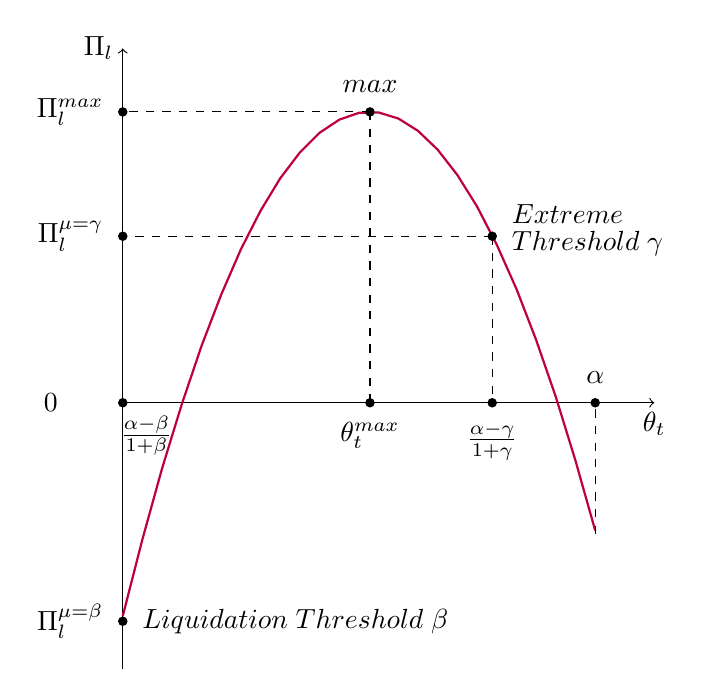
\begin{tikzpicture}[scale=0.75]

\draw[<->] (9,0) node[below]{$\theta_t$} -- (0,0) node[left]{$0 \quad \quad$} -- (0,6) node[left]{$\Pi_l$};
\draw[-] (0,0)  -- (0,-4.5) ;
\draw[purple, thick, domain=0:8] plot (\x, {-12480*((\x/160+0.05)-0.0562962)*((\x/160+0.05)-0.0960265)});

\draw [dashed] (4.185816,4.92494) -- (4.185816,0);
\draw [dashed] (4.185816,4.92494) -- (0,4.92494);   
\draw [dashed] (8,-2.22) -- (8,0);   
\draw [dashed] (6.256,2.82) -- (0,2.82);   
\draw [dashed] (6.256,2.82) -- (6.256,0);   

\filldraw[black](0,0) circle (2pt) node[dotted,label=below:{$\frac{\alpha - \beta}{1+ \beta}$}]  at (0.4,0.1) (int0) {};
\filldraw[black](4.185816,4.92494) circle (2pt) node[dotted,label=above:$max$] (int1) {};
\filldraw[black](4.185816,0) circle (2pt) node[dotted,label=below:{$\theta_t^{max}$}] (int2) {};
\filldraw[black](0,4.92494) circle (2pt) node[dotted,label=left:$\Pi_l^{max}$]  (int3) {};
\filldraw[black] (8,0) circle (2pt) node[dotted,label=above:{$\alpha$}] (int4) {};
\filldraw[black] (6.256,0) circle (2pt) node[dotted,label=below:{$\frac{\alpha - \gamma}{1+ \gamma}$}] (int5) {};

\filldraw[black](6.256,2.82) circle (2pt) {};
\filldraw[black](0,2.82) circle (2pt) node[dotted,label=left:{$\Pi_l^{\mu=\gamma}$}]  (int6) {};
\filldraw[black](0,-3.7) circle (2pt) node[dotted,label=right:{$Liquidation \; Threshold \; \beta$}] (int7a) {};

\node[dotted,label=left:{$\Pi_l^{\mu=\beta}$}] at (0,-3.7) (int7b) {};
\node[dotted,label=right:{$Extreme$}] at (6.256,3.2) (int8) {};
\node[dotted,label=right:{$Threshold \; \gamma$}] at (6.256,2.7) (int9) {};

\end{tikzpicture}
\end{center}

\vspace{5mm}

\begin{center}
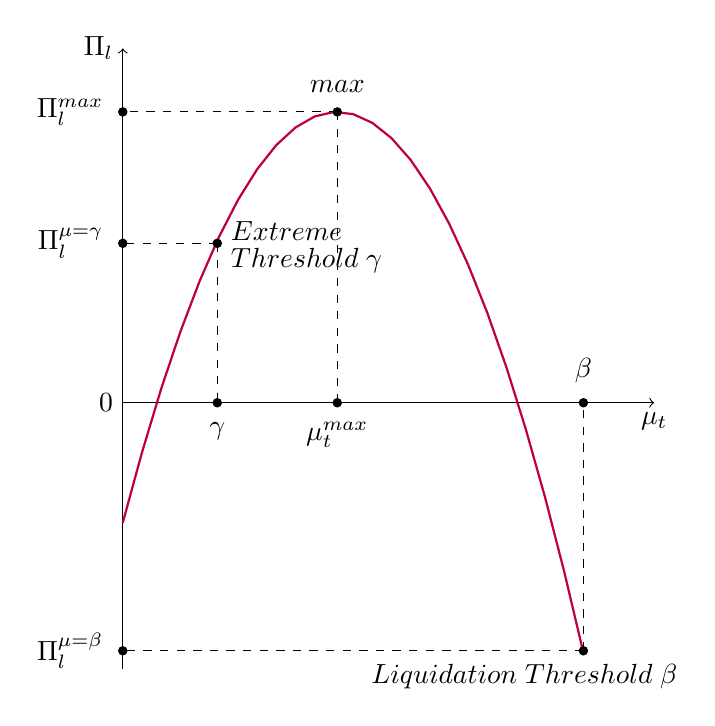
\begin{tikzpicture}[scale=0.75]

\draw[<->] (9,0) node[below]{$\mu_t$} -- (0,0) node[left]{$0$} -- (0,6) node[left]{$\Pi_l$};
\draw[-] (0,0)  -- (0,-4.5) ;
\draw[purple, thick, domain=0:7.8] plot (\x, {-2.0315 + 3.8306*\x - 0.5273*\x*\x});

\draw [dashed] (3.632,4.92494) -- (3.632,0);
\draw [dashed] (3.632,4.92494) -- (0,4.92494);   
\draw [dashed] (7.8,-4.2) -- (7.8,0);   
\draw [dashed] (1.6,2.7) -- (0,2.7);   
\draw [dashed] (1.6,2.7) -- (1.6,0);   
\draw [dashed] (7.8,-4.2) -- (0,-4.2);   

\filldraw[black](3.632,4.92494) circle (2pt) node[dotted,label=above:$max$] (int1) {};
\filldraw[black](3.632,0) circle (2pt) node[dotted,label=below:{$\mu_t^{max}$}] (int2) {};
\filldraw[black](0,4.92494) circle (2pt) node[dotted,label=left:$\Pi_l^{max}$]  (int3) {};
\filldraw[black] (7.8,0) circle (2pt) node[dotted,label=above:{$\beta$}] (int4) {};
\filldraw[black](1.6,0) circle (2pt) node[dotted,label=below:{$\gamma$}] (int5) {};
\filldraw[black](0,-4.2) circle (2pt)  {};
\filldraw[black](7.8,-4.2) circle (2pt) {};
\filldraw[black](0,2.7) circle (2pt) node[dotted,label=left:{$\Pi_l^{\mu=\gamma}$}]  (int6) {};
\filldraw[black](1.6,2.7) circle (2pt) {};

\node[dotted,label=right:{$Extreme$}] at (1.5,2.9) (int6u) {};
\node[dotted,label=right:{$Threshold \; \gamma$}] at (1.5,2.4) (int6d){};
\node[dotted,label=below:{$Liquidation \; Threshold \; \beta$}] at (6.8,-4.1)(int7a) {};
\node[dotted,label=left:{$\Pi_l^{\mu=\beta}$}] at (0,-4.2) (int7b) {};

\end{tikzpicture}
\end{center}

\newpage
For $\alpha = 10\%$, $\beta = 5\%$, $\gamma = 1\%$, $a_t=0.5\%$, $b_t=0.5\%$, $v=1,000$ and $m_0=1.2$, when $\mu_t\in [\gamma,\beta]$, we have $\mu_t^{max}=2.25\%$, $\theta_t^{max}=7.6\%$ and $\Pi_l^{max}=11.5$ USD stablecoins.


\begin{center}
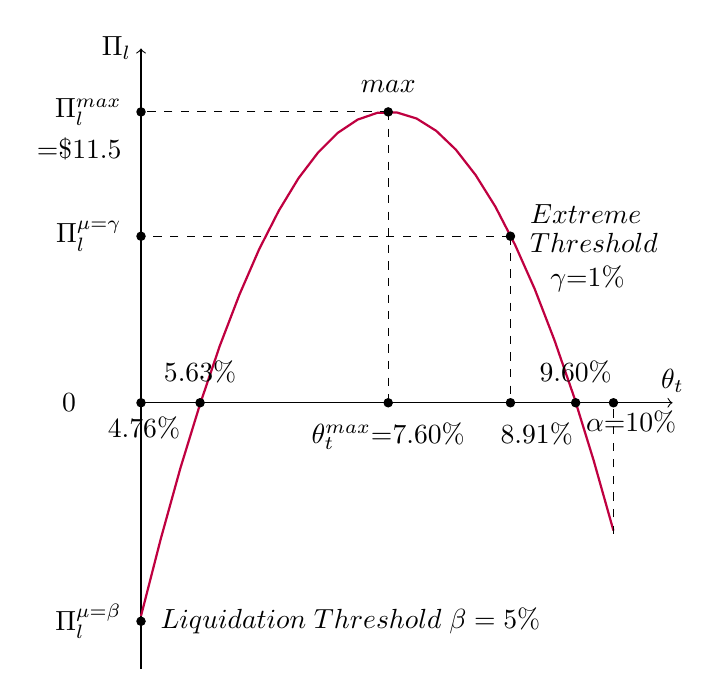
\begin{tikzpicture}[scale=0.75]

\draw[<->] (9,0) node[above]{$\theta_t$} -- (0,0) node[left]{$0 \quad \quad$} -- (0,6) node[left]{$\Pi_l$};
\draw[-] (0,0)  -- (0,-4.5) ;
\draw[purple, thick, domain=0:8] plot (\x, {-12480*((\x/160+0.05)-0.0562962)*((\x/160+0.05)-0.0960265)});

\draw [dashed] (4.185816,4.92494) -- (4.185816,0);
\draw [dashed] (4.185816,4.92494) -- (0,4.92494);   
\draw [dashed] (8,-2.22) -- (8,0);   
\draw [dashed] (6.256,2.82) -- (0,2.82);   
\draw [dashed] (6.256,2.82) -- (6.256,0);   

\filldraw[black](0,0) circle (2pt) node[dotted,label=below:{$4.76\%$}]  at (0.05,0.1) (int0) {};
\filldraw[black](4.185816,4.92494) circle (2pt) node[dotted,label=above:$max$] (int1) {};
\filldraw[black](4.185816,0) circle (2pt) node[dotted,label=below:{$\theta_t^{max}$=$7.60\%$}] (int2) {};
\filldraw[black](0,4.92494) circle (2pt) node[dotted,label=left:$\Pi_l^{max}$]  (int3) {};
\filldraw[black] (8,0) circle (2pt) node[dotted,label=below:{$\alpha$=$10\%$}] at (8.3,0.2) (int4) {};
\filldraw[black] (6.256,0) circle (2pt) node[dotted,label=below:{$8.91\%$}] at (6.7,0) (int5) {};

\filldraw[black] (1,0) circle (2pt) node[dotted,label=above:{$5.63\%$}] at (1,0) (int5a) {};
\filldraw[black] (7.36,0) circle (2pt) node[dotted,label=above:{$9.60\%$}] at (7.36,0) (int5b) {};

\filldraw[black](6.256,2.82) circle (2pt) {};
\filldraw[black](0,2.82) circle (2pt) node[dotted,label=left:{$\Pi_l^{\mu=\gamma}$}]  (int6) {};
\filldraw[black](0,-3.7) circle (2pt) node[dotted,label=right:{$Liquidation \; Threshold \; \beta=5\%$}] (int7a) {};

\node[dotted,label=left:{$\Pi_l^{\mu=\beta}$}] at (0,-3.7) (int7b) {};
\node[dotted,label=right:{$Extreme$}] at (6.256,3.2) (int8) {};
\node[dotted,label=right:{$Threshold$}] at (6.256,2.7) (int9) {};
\node[dotted,label=right:{$\gamma$=$1\%$}] at (6.6,2.1) (int10) {};

\node[dotted,label=left:{=$\$11.5$}] at (0,4.3) (int11) {};

\end{tikzpicture}
\end{center}

\begin{center}
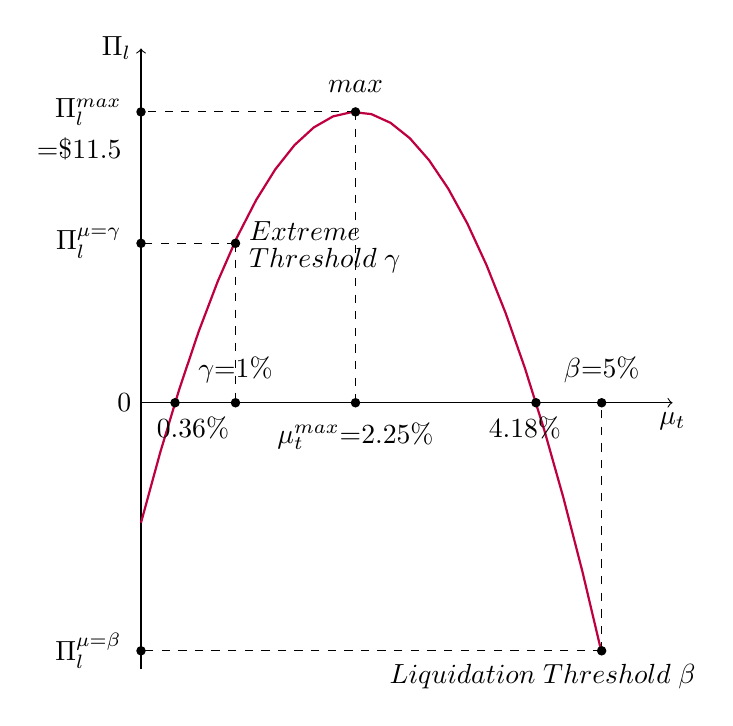
\begin{tikzpicture}[scale=0.75]

\draw[<->] (9,0) node[below]{$\mu_t$} -- (0,0) node[left]{$0$} -- (0,6) node[left]{$\Pi_l$};
\draw[-] (0,0)  -- (0,-4.5) ;
\draw[purple, thick, domain=0:7.8] plot (\x, {-2.0315 + 3.8306*\x - 0.5273*\x*\x});

\draw [dashed] (3.632,4.92494) -- (3.632,0);
\draw [dashed] (3.632,4.92494) -- (0,4.92494);   
\draw [dashed] (7.8,-4.2) -- (7.8,0);   
\draw [dashed] (1.6,2.7) -- (0,2.7);   
\draw [dashed] (1.6,2.7) -- (1.6,0);   
\draw [dashed] (7.8,-4.2) -- (0,-4.2);   

\filldraw[black](3.632,4.92494) circle (2pt) node[dotted,label=above:$max$] (int1) {};
\filldraw[black](3.632,0) circle (2pt) node[dotted,label=below:{$\mu_t^{max}$=2.25\%}]  (int2) {};
\filldraw[black](0,4.92494) circle (2pt) node[dotted,label=left:$\Pi_l^{max}$] (int3) {};
\filldraw[black] (7.8,0) circle (2pt) node[dotted,label=above:{$\beta$=$5\%$}]  (int4) {};
\filldraw[black] (0.576,0) circle (2pt) node[dotted,label=below:{$0.36\%$}] at (0.88,0.1) (int5) {};
\filldraw[black] (6.688,0) circle (2pt) node[dotted,label=below:{$4.18\%$}] at (6.5,0.1) (int5a) {};
\filldraw[black](1.6,0) circle (2pt) node[dotted,label=above:{$\gamma$=$1\%$}] (int5b) {};

\filldraw[black](0,-4.2) circle (2pt)  {};
\filldraw[black](7.8,-4.2) circle (2pt) {};
\filldraw[black](0,2.7) circle (2pt) node[dotted,label=left:{$\Pi_l^{\mu=\gamma}$}]  (int6) {};
\filldraw[black](1.6,2.7) circle (2pt) {};

\node[dotted,label=right:{$Extreme$}] at (1.5,2.9) (int6u) {};
\node[dotted,label=right:{$Threshold \; \gamma$}] at (1.5,2.4) (int6d){};
\node[dotted,label=below:{$Liquidation \; Threshold \; \beta$}] at (6.8,-4.1)(int7a) {};
\node[dotted,label=left:{$\Pi_l^{\mu=\beta}$}] at (0,-4.2) (int7b) {};
\node[dotted,label=left:{=$\$11.5$}] at (0,4.3) (int8) {};

\end{tikzpicture}
\end{center}


After the position is liquidated by a liquidator, the liquidity provider receives the remaining proportion of the collateral, 
$$(1-\delta)(c_t + b_t m_t v)>0$$
and make a loss of
$$(1-\delta)(c_t + b_t m_t v) - (\alpha-a_0)m_0v<0$$

\section{One Position in One Liquidity Pool}
As traders place the first, second, third, $i_{th}$ to $n_{th}$ trade orders to buy fEUR tokens, open positions are created at each order as collateral. While in reality, liquidity provider of a liquidity pool combines all positions together and holds only one position that for total open unit of fEUR tokens
$$V=\sum_{i=1}^n v^i=v^1+v^2+v^3+...+v^n$$

Total collateral that belong to the liquidity provider
$$C_t=\sum_{i=1}^n c_t^i = \sum_{i=1}^n \mu_t^i m_t v_t^i= \sum_{i=1}^n (\alpha - \theta_t^i)m_0^i v^i$$

as ratio of liquidity provider's collateral to the current value of all minted fEUR tokens backed up by the pool
$$ M_t=\frac{C_t}{m_t V}$$

Note that $M_t$ is a weighted average of $\mu_t^i$ as 
$$ M_t=\sum_{i=1}^n  \frac{v_t^i}{V} \mu_t^i$$

Now when $M_t \in [\gamma,\beta]$, i.e. the liquidity provider collateral ratio falls in between the Extreme Threshold and Liquidation Threshold, any liquidator is allowed to liquidate a fraction or the entire open position in the pool, by

\begin{itemize}

    \item Buy $\rho V$ fEUR tokens from any liquidity provider at cost $(1+a_t)m_t \rho V$ or at any exchange at a similar cost, where $\rho \in (0,1]$ represent the fraction of the open position that liquidator would like to close. 
    
    \item Deposit the tokens into the liquidity pool to close the position (by selling the exact amount of fEUR tokens at bid price $(1-b_t)m_t$ back to close the original open position) and receive the sale return of the fEUR tokens plus \textbf{\textit{some proportion}} of the collateral belongs to the liquidity provider in the fraction of the position and the income from bid spread at close of the fraction of the position:
    $$(1-b_t)m_t \rho V + \delta(\rho C_t + b_t m_t \rho V)$$
    where $\delta$ is the proportion of Liquidity Provider's collateral to be given to the liquidator if a position is liquidated that $$ \delta_t=\frac{\lambda_t}{\beta-\gamma}=\frac{\beta-M_t}{\beta-\gamma}$$
    and $\lambda$ represents how far away the current Liquidity Provider's collateral ratio is from the Liquidation Threshold that $$\lambda_t=\beta-M_t$$
    
    \begin{center}
    \begin{tikzpicture}[scale=0.9]

    \draw[<->] (9,0) node[below]{$\lambda(M_t)$} -- (0,0) -- (0,6) node[left]{$\delta(M_t)$};
    \draw [thick, blue] (0,0) -- (7.5,4.5);
    \draw [dashed] (7.5,4.5) -- (7.5,0);
    \draw [dashed] (7.5,4.5) -- (0,4.5);   

    \node[dotted,label=left:$0$] at (0,0) (int0) {};
    \node[dotted,label=below:$\beta-\gamma$] at (7.5,0) (int1) {};
    \node[dotted,label=left:$100\%$] at (0,4.5) (int2) {};
    \node[dotted,label=below:{$\delta=\frac{\lambda}{\beta - \gamma}$}] at (6,3.3) (int3) {};

    \end{tikzpicture}
    \end{center}

    \item Make profit 
    $$ \Pi_l = [b_t(\delta - 1) - a_t] m_t \rho V + \delta \rho C_t $$ 
    if his tokens are purchased from a liquidity provider. 
    \vspace{5mm} 

    Since 
    $$\delta_t=\frac{\beta - M_t}{\beta -\gamma}$$
    $$C_t= m_t V M_t$$
    $$m_t=\frac{(\alpha + 1)\sum_{i=1}^n m_0^i v^i }{(M_t+1)V}$$
    
    $$\Pi_l(M_t) = \left[\frac{(b_t + M_t) (\beta -M_t)}{\beta - \gamma}  - (a_t+b_t)  \right] \frac{(\alpha +1) \rho \sum_{i=1}^n m_0^i v^i}{M_t + 1}$$
    
    For $M_t \in [\gamma,\beta]$, there exists a local maxima solution $$M_t^{max}(m_0^i,v^i,\alpha,\beta,\gamma,a_t,b_t)$$ 
    
    that generate maximized profit
    $$\Pi_l^{max}(\rho, M_t^{max})$$
    when 
    $$\frac{\partial \Pi_l}{\partial M_t}=0$$
\vspace{5mm} 

\begin{center}
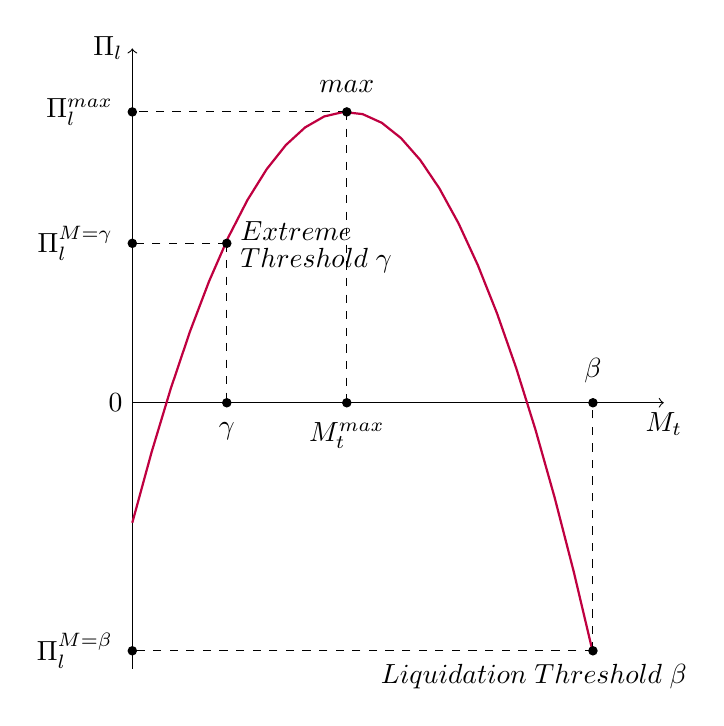
\begin{tikzpicture}[scale=0.75]

\draw[<->] (9,0) node[below]{$M_t$} -- (0,0) node[left]{$0$} -- (0,6) node[left]{$\Pi_l$};
\draw[-] (0,0)  -- (0,-4.5) ;
\draw[purple, thick, domain=0:7.8] plot (\x, {-2.0315 + 3.8306*\x - 0.5273*\x*\x});

\draw [dashed] (3.632,4.92494) -- (3.632,0);
\draw [dashed] (3.632,4.92494) -- (0,4.92494);   
\draw [dashed] (7.8,-4.2) -- (7.8,0);   
\draw [dashed] (1.6,2.7) -- (0,2.7);   
\draw [dashed] (1.6,2.7) -- (1.6,0);   
\draw [dashed] (7.8,-4.2) -- (0,-4.2);   

\filldraw[black](3.632,4.92494) circle (2pt) node[dotted,label=above:$max$] (int1) {};
\filldraw[black](3.632,0) circle (2pt) node[dotted,label=below:{$M_t^{max}$}] (int2) {};
\filldraw[black](0,4.92494) circle (2pt) node[dotted,label=left:$\Pi_l^{max}$]  (int3) {};
\filldraw[black] (7.8,0) circle (2pt) node[dotted,label=above:{$\beta$}] (int4) {};
\filldraw[black](1.6,0) circle (2pt) node[dotted,label=below:{$\gamma$}] (int5) {};
\filldraw[black](0,-4.2) circle (2pt)  {};
\filldraw[black](7.8,-4.2) circle (2pt) {};
\filldraw[black](0,2.7) circle (2pt) node[dotted,label=left:{$\Pi_l^{M=\gamma}$}]  (int6) {};
\filldraw[black](1.6,2.7) circle (2pt) {};

\node[dotted,label=right:{$Extreme$}] at (1.5,2.9) (int6u) {};
\node[dotted,label=right:{$Threshold \; \gamma$}] at (1.5,2.4) (int6d){};
\node[dotted,label=below:{$Liquidation \; Threshold \; \beta$}] at (6.8,-4.1)(int7a) {};
\node[dotted,label=left:{$\Pi_l^{M=\beta}$}] at (0,-4.2) (int7b) {};

\end{tikzpicture}
\end{center}

\newpage

    For $\alpha = 10\%$, $\beta = 5\%$, $\gamma = 1\%$, $a_t=0.5\%$, $b_t=0.5\%$, $\sum_{i=1}^n m_0^i v^i=6,000$ and $\rho =20\%$, when $M_t\in [\gamma,\beta]$, we have $M_t^{max}=2.25\%$ and $\Pi_l^{max}=11.5$ USD stablecoins.
    
   \vspace{5mm}
   
\begin{center}
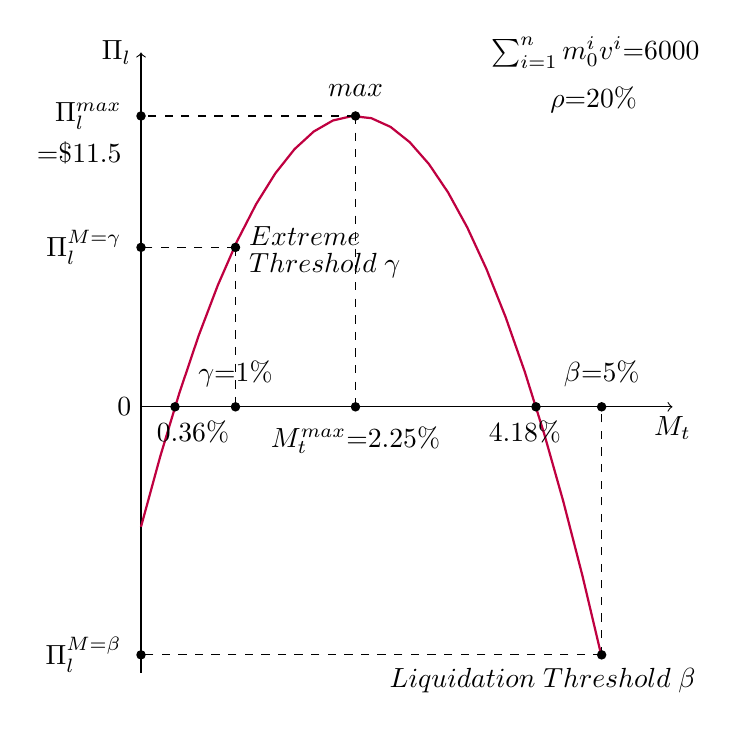
\begin{tikzpicture}[scale=0.75]

\draw[<->] (9,0) node[below]{$M_t$} -- (0,0) node[left]{$0$} -- (0,6) node[left]{$\Pi_l$};
\draw[-] (0,0)  -- (0,-4.5) ;
\draw[purple, thick, domain=0:7.8] plot (\x, {-2.0315 + 3.8306*\x - 0.5273*\x*\x});

\draw [dashed] (3.632,4.92494) -- (3.632,0);
\draw [dashed] (3.632,4.92494) -- (0,4.92494);   
\draw [dashed] (7.8,-4.2) -- (7.8,0);   
\draw [dashed] (1.6,2.7) -- (0,2.7);   
\draw [dashed] (1.6,2.7) -- (1.6,0);   
\draw [dashed] (7.8,-4.2) -- (0,-4.2);   

\filldraw[black](3.632,4.92494) circle (2pt) node[dotted,label=above:$max$] (int1) {};
\filldraw[black](3.632,0) circle (2pt) node[dotted,label=below:{$M_t^{max}$=2.25\%}]  (int2) {};
\filldraw[black](0,4.92494) circle (2pt) node[dotted,label=left:$\Pi_l^{max}$] (int3) {};
\filldraw[black] (7.8,0) circle (2pt) node[dotted,label=above:{$\beta$=$5\%$}]  (int4) {};
\filldraw[black] (0.576,0) circle (2pt) node[dotted,label=below:{$0.36\%$}] at (0.88,0.1) (int5) {};
\filldraw[black] (6.688,0) circle (2pt) node[dotted,label=below:{$4.18\%$}] at (6.5,0.1) (int5a) {};
\filldraw[black](1.6,0) circle (2pt) node[dotted,label=above:{$\gamma$=$1\%$}] (int5b) {};

\filldraw[black](0,-4.2) circle (2pt)  {};
\filldraw[black](7.8,-4.2) circle (2pt) {};
\filldraw[black](0,2.7) circle (2pt) node[dotted,label=left:{$\Pi_l^{M=\gamma}$}]  (int6) {};
\filldraw[black](1.6,2.7) circle (2pt) {};

\node[dotted,label=right:{$Extreme$}] at (1.5,2.9) (int6u) {};
\node[dotted,label=right:{$Threshold \; \gamma$}] at (1.5,2.4) (int6d){};
\node[dotted,label=below:{$Liquidation \; Threshold \; \beta$}] at (6.8,-4.1)(int7a) {};
\node[dotted,label=left:{$\Pi_l^{M=\beta}$}] at (0,-4.2) (int7b) {};
\node[dotted,label=left:{=$\$11.5$}] at (0,4.3) (int8) {};

\node[dotted,label=right:{$\sum_{i=1}^n m_0^i v^i$=$6000$}] at (5.6,6) (int9) {};
\node[dotted,label=right:{$\rho$=$20\%$}] at (6.6,5.2) (int10) {};

\end{tikzpicture}
\end{center}


\end{itemize}


After the $\rho$ fraction of the position is liquidated by a liquidator, the liquidity provider receives the remaining fraction of spread income from buying back fEUR tokens $(1-\delta)b_t m_t \rho V$, and keeps the remaining fraction of collateral of the closed position $(1-\delta) \rho C_t$. And the new position becomes 
$$\{(1-\rho)m_t V \quad \quad + \quad \quad C_t (1-\delta \rho) + (1-\delta)b_t m_t \rho V\}$$
and the new liquidity provider collateral ratio
$$M_t^{new}=\frac{C_t^{new}}{V^{new}} =\frac{C_t^{old}(1-\delta \rho) + (1-\delta)b_t m_t \rho V}{(1-\rho)m_t V}>M_t^{old}$$

- If $M_t^{new}>\beta$, there will be no immediate arbitrage opportunity. \par
- While if we still have $M_t^{new} \leq \beta$, any liquidator can keep closing more fraction of the open position, until reaching $M_t>\beta$, i.e. when the current liquidity provider collateral ratio exceeds the Liquidation Threshold.


\end{document}